\section{Исследование влияния широтно-импульсной модуляции на качество проектируемой системы}
Существенное влияние на свойства разрабатываемой системы управления могут ввести особенности технической реализации управляющего устройства. В частности, при высоком уровне энергии в управляемом объекте реализация управляющих воздействий в виде непрерывных сигналов практически невозможна в силу больших потерь в выходных каскадах исполнительных устройств. В таких случаях выходные каскады выполняют в виде импульсных устройств, в которых непрерывный сигнал квантуется по уровню или по времени, а затем преобразуется в импульсную модулированную последовательность. Одним из видов модуляции является широтно-импульсная (ШИМ), при которой непрерывный сигнал преобразуется в последовательность импульсов одинаковой амплитуды при постоянном периоде повторения Т, а длительность импульса определяется по какому-либо закону, например, линейному, в зависи¬мости от значения входного модулируемого непрерывного сигнала.

Управляющий сигнал формируется компаратором, когда на его инвертирующий вход подается пилообразный сигнал, а на неинвертирующий — модулирующий непрерывный сигнал. Выходные импульсы получаются прямоугольными, частота их следования равна частоте пилы, а длительность положительной части импульса связана с временем, в течение которого уровень модулирующего сигнала, подаваемого на неинвертирующий вход компаратора, оказывается выше уровня сигнала пилы, который подается на инвертирующий вход. Когда напряжение пилы выше модулирующего сигнала, на выходе будет отрицательная часть импульса.

Следует отметить, что при смене полярности модулируемого сигнала полярность импульсов также меняется. Длительность импульсов на выходе модулятора может меняться от нуля до непрерывного сигнала, при этом амплитуда и период повторения (частота) следования импульсов остаются неизменными.

\clearpage
\subsection{ШИМ}
ШИМ на  рис.\ref{fig:sim_final_VSS_PWM}. 
\begin{figure}[!h]\centering
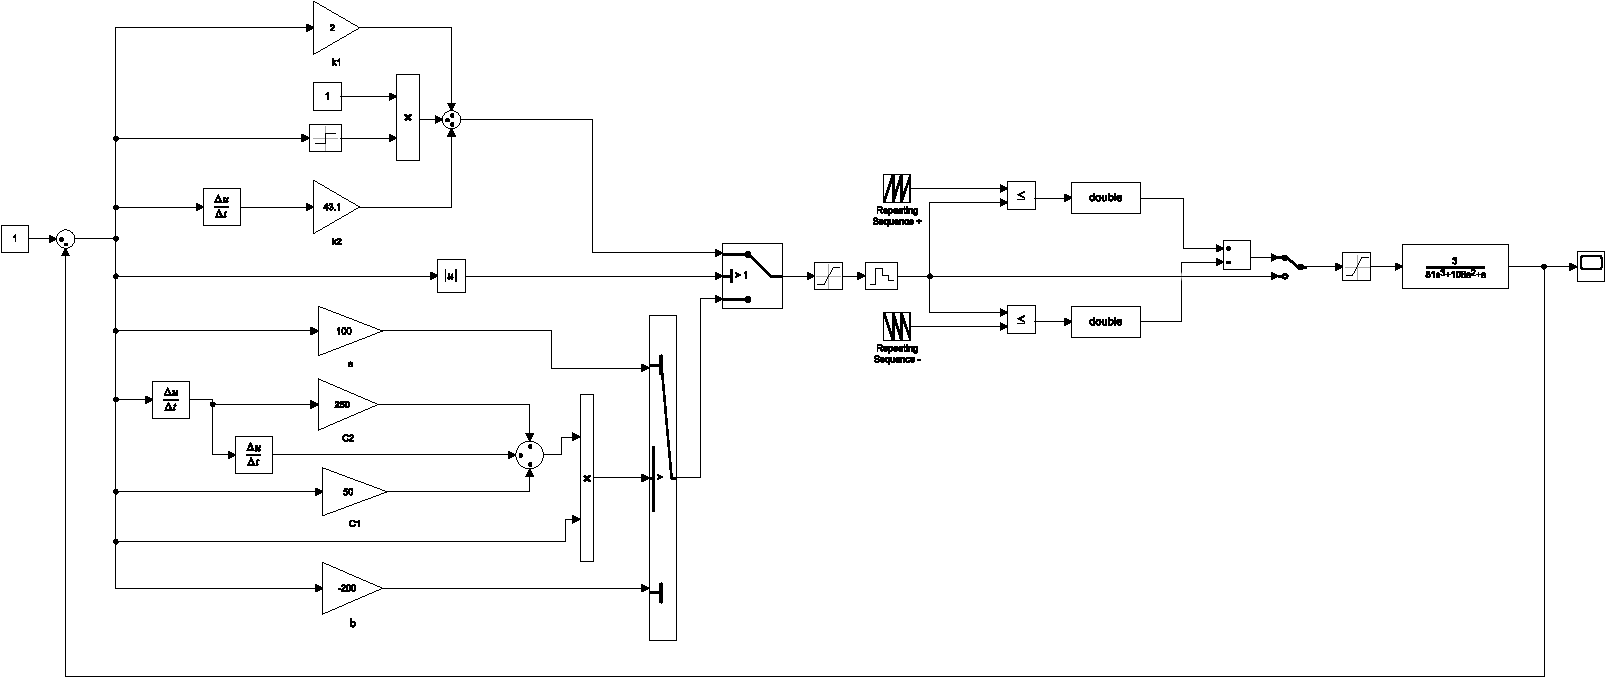
\includegraphics[width=1.0\linewidth]{images/sim_final_VSS_PWM}
\caption{Структурная схема нелинейной СПС с ШИМ. }\label{fig:sim_final_VSS_PWM}
\end{figure}

в результате видим, что переходный процесс не изменился
\begin{figure}[!h]\centering
\includegraphics[width=0.6\linewidth]{images/final_VSS_PWM_DCS_SAWnew}
\caption{ Переворачиваем пилу  и поднимаем её над осью абсцис}\label{fig:final_VSS_PWM_DCS_SAWnew}
\end{figure}
\begin{figure}[!h]\centering
\includegraphics[width=0.6\linewidth]{images/final_VSS_PWM_DCS_pwm1}
\caption{ ШИМ1}\label{fig:final_VSS_PWM_DCS_pwm1}
\end{figure}
\begin{figure}[!h]\centering
\includegraphics[width=0.6\linewidth]{images/final_VSS_PWM_DCS_pwm2}
\caption{ ШИМ2}\label{fig:final_VSS_PWM_DCS_pwm2}
\end{figure}
\begin{figure}[!h]\centering
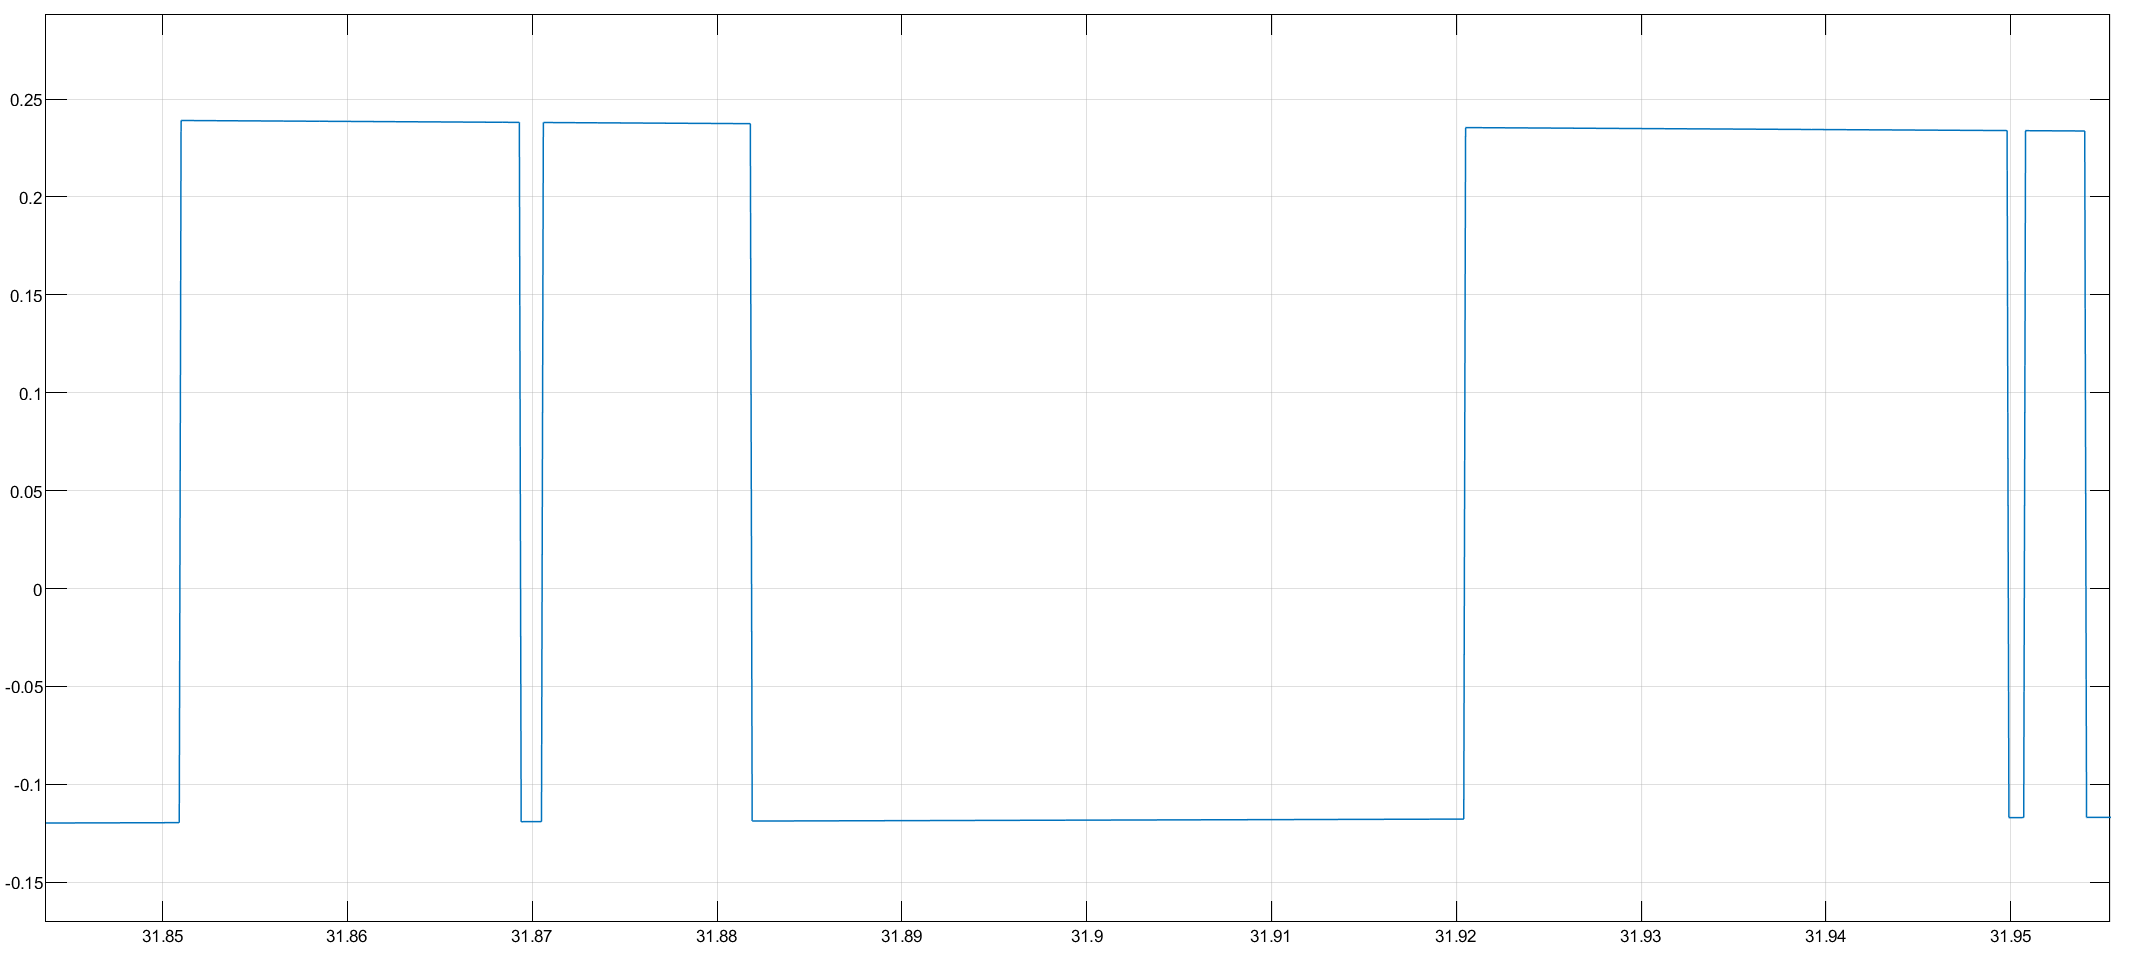
\includegraphics[width=0.6\linewidth]{images/final_VSS_PWM_DCS_upr}
\caption{ управляющий непрерывный сигнал }\label{fig:final_VSS_PWM_DCS_upr}
\end{figure}
\begin{figure}[!h]\centering
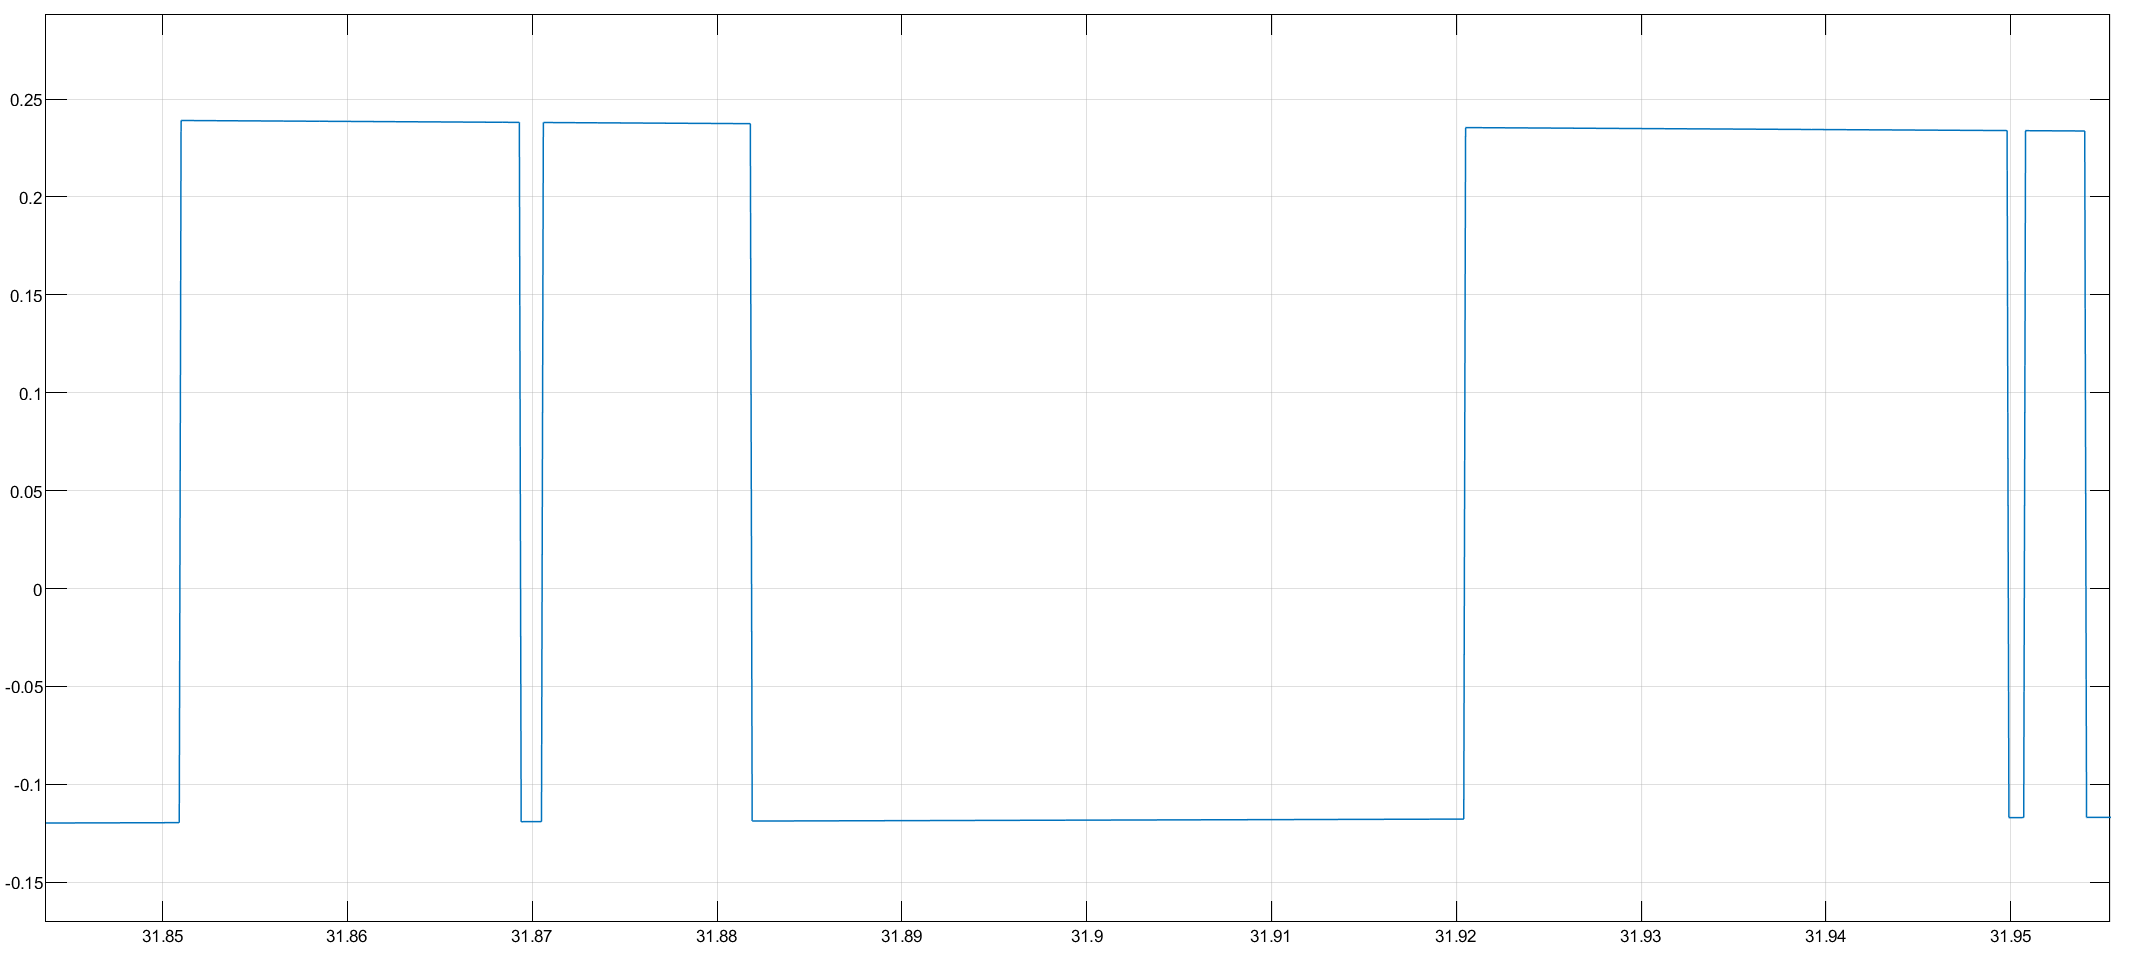
\includegraphics[width=0.6\linewidth]{images/final_VSS_PWM_DCS_upr_ogr}
\caption{ управляющий непрерывный сигнал после насыщения}\label{fig:final_VSS_PWM_DCS_upr_ogr}
\end{figure}


